% Urban Leak Monitoring Dashboard — research paper
% Build: pdflatex urban-leak-monitoring.tex (twice). Figures in figures/.

\documentclass[11pt,a4paper]{article}
\usepackage[utf8]{inputenc}
\usepackage[T1]{fontenc}
\usepackage{lmodern}
\usepackage{microtype}
\usepackage[margin=2.5cm]{geometry}
\usepackage{booktabs}
\usepackage{array}
\usepackage{parskip}
\usepackage{enumitem}
\usepackage{graphicx}
\usepackage{subcaption}
\usepackage{xcolor}
\usepackage{amsmath}
\usepackage[hidelinks]{hyperref}
\usepackage{url}
\usepackage{xurl}

\linespread{1.08}
\graphicspath{{figures/}}
\setlist{itemsep=2pt,topsep=4pt}

\newcommand{\appname}{Urban Leak Monitoring Dashboard}
\newcommand{\repourl}{https://github.com/suadarzimanli/water-leak-monitoring-dashboard}
\newcommand{\appurl}{https://suadarzimanli.github.io/water-leak-monitoring-dashboard/}
\newcommand{\archivedoi}{}

\title{Context Before Dispatch: Leak Alarms and Look-Alike Events\\ in a Simulated Water Distribution Network}
\author{Suad Arzimanli\\[2pt]
        \small University of \L{}ód\'{z}, Faculty of Mathematics and Computer Science, Poland\\
        \small \texttt{suad.arzimanli@gmail.com}}
\date{}

\begin{document}
\maketitle

\begin{abstract}
Water utilities detect leaks by watching hourly flow and pressure in district metered areas, but many alarms are false: scheduled hydrant tests, valve work, hot-weather demand and faulty sensors produce the same signature as a leak. This paper asks how much of that false-alarm burden detection methods can remove, and where the information that removes it actually lies. I built a simulator of eight pressure zones with a two-peak daily demand profile, weather, published maintenance, unscheduled hydrant use, pressure-sensor drift and leaks that persist until repaired, and compared three detectors on 40 simulated networks with 400 test leaks: robust threshold rules, a logistic regression on deviations from hourly baselines, and the same model followed by a context check that uses only information an operator has --- the published schedule, the day's weather and whether pressure fits the observed flow.

With an alert raised after two consecutive abnormal hours, the rules detected 308 of 400 leaks at 0.41 false alerts per zone-week; the learned model detected 376 but raised 1.02 false alerts per zone-week; the model with the context check detected 369 at 0.19 false alerts per zone-week, removing 81\% of the model's false alerts (95\% interval of the difference $-1.01$ to $-0.67$) at a cost of seven leaks. Training the model with the look-alike events as negative examples did not reduce its false alerts: their flow and pressure signatures are indistinguishable from leaks, and the information that separates them is in the schedule and the weather, not in the readings. The study is implemented as an open-source teaching dashboard in which operators work each incident from alert to close-out and see the simulated truth only after deciding.

\medskip
\noindent\textbf{Keywords:} leak detection; water distribution; SCADA; false alarms; district metered areas; human-in-the-loop monitoring; simulation study.

\smallskip
\noindent\textbf{Disclaimer.} Educational simulation. Zones are placed on an OpenStreetMap basemap for illustration only; zone names, the network and all readings are fictional. Not affiliated with, endorsed by, or based on data from any water utility or public authority.
\end{abstract}

%======================================================================
\section{Introduction}

A substantial share of treated drinking water never reaches customers; leaks from mains and service pipes are the largest physical component of these losses \cite{lambert2002,farley2003}. Utilities therefore divide networks into district metered areas (DMAs) and monitor their inflow and pressure, looking for the classic leak signature: more flow than usual, together with lower pressure \cite{puust2010,farley2003}. Data-driven burst detection on such telemetry has matured into operational systems \cite{mounce2010,romano2014,wu2017}.

The practical difficulty is not only detecting leaks but deciding which alarms deserve a crew. Many events change flow and pressure in the same direction as a leak: scheduled hydrant flushing and flow tests, valve operations, high demand on hot days and drifting pressure transmitters. A detector that flags all of them produces false alerts that operators learn to ignore --- the alarm-fatigue problem known from other monitoring domains \cite{cvach2012} --- while operators who over-trust an automated detector may dispatch crews to non-events \cite{parasuraman1997,bainbridge1983}.

This paper studies that problem in a controlled simulation. Real SCADA data with confirmed leak labels are rarely public, so a simulator lets every event be known and every method be compared on identical streams. The study is embedded in an interactive dashboard that teaches the operator's side: each incident is worked through acknowledgement, work order, dispatch and close-out, and the simulated truth is revealed only after the decision.

\subsection{Research questions}

\begin{description}[leftmargin=2.6em,style=nextline]
  \item[RQ1] How do threshold rules and a learned model compare in leaks detected and false alerts when leak-like operational events are present?
  \item[RQ2] Does training the model with the look-alike events as negative examples reduce its false alerts?
  \item[RQ3] How many false alerts does a context check using only operator-visible information remove, and at what cost in missed leaks?
  \item[RQ4] How can a dashboard teach the path from alarm to close-out without revealing what the operator could not know?
\end{description}

\subsection{Contributions}

\begin{enumerate}
  \item A transparent, seeded \textbf{network simulator} with persistent leaks and five kinds of look-alike events (\S\ref{sec:sim}).
  \item A \textbf{comparison of four detectors} on 40 networks with a separate set of design networks, three alert-persistence settings, paired bootstrap intervals and an attribution of every false alert to its cause (\S\ref{sec:eval}--\S\ref{sec:results}).
  \item An \textbf{operator-visible context check} that removes most false alerts of a learned detector (\S\ref{sec:detect}).
  \item An open-source \textbf{teaching dashboard} sharing its code with the study, so the numbers it displays are computed exactly as in this paper (\S\ref{sec:app}).
\end{enumerate}

%======================================================================
\section{Background}

\paragraph{Leakage management.} Leakage management combines active leak detection, pressure management, speed and quality of repairs and asset renewal \cite{farley2003,puust2010}. Within a DMA, minimum night flow is a traditional indicator because legitimate demand is lowest at night, so sustained extra flow then points to leakage \cite{farley2003}. Breaks of mains are more frequent in cold weather \cite{kleiner2001}. Hydraulic and transient-based methods can localise leaks along pipes \cite{colombo2009}; this study works at the coarser level of zone telemetry.

\paragraph{Data-driven burst detection.} Statistical and machine-learning detectors compare observed flow and pressure with a predicted or historical baseline and raise an alarm when the deviation is large and persistent \cite{mounce2010,romano2014}. Reviews note that published methods are evaluated on few, often private datasets with inconsistent measures, and that false alarms from operational events remain a key obstacle to deployment \cite{wu2017}. When the event of interest is rare, precision and recall are more informative than accuracy or ROC curves \cite{saito2015}.

\paragraph{Operators and automation.} Automation changes rather than removes the human role: operators must monitor the automation and take over in exactly the hard cases \cite{bainbridge1983}. Trust in an alarm system follows its reliability; frequent false alarms lead to disuse, and imperfect diagnostic aids help only when they are reliable enough \cite{parasuraman1997,wickens2007}. These findings motivate measuring false alerts per unit of time, which is what an operator experiences, and keeping the information behind an alert visible.

%======================================================================
\section{Simulated network}
\label{sec:sim}

The network has eight pressure zones with base flows of 86--115\,L/s and base pressures of 55--63\,psi. Every hour each zone reports flow and pressure. Demand follows a daily profile with a minimum around 02:00, a morning peak around 08:00 and an evening peak around 19:00 (factors 0.73, 1.34 and 1.23 of the daily mean). Pressure falls with demand through head loss (0.06\,psi per L/s). Sensor noise has a standard deviation of 2.5\,L/s for flow and 0.7\,psi for pressure. Each day has a weather type: clear (55\%), rain (20\%; demand $-6\%$), heat (15\%; demand $+8\%$) or cold (10\%; break risk $\times 2.2$).

Table~\ref{tab:events} lists the events. Leaks and look-alike events add flow and reduce pressure; what distinguishes a leak is mainly that it persists and that its pressure drop per unit of extra flow is larger than demand would cause --- but scheduled valve work has a similar ratio, and hydrant use adds far more flow. Scheduled hydrant tests and valve work are published in a schedule before they happen, as utilities do with planned work. Every random stream (weather, schedule, events per zone, noise per zone) is seeded separately, so a seed fully determines a network and a live continuation is consistent with its history.

\begin{table}[htbp]
\centering
\small
\caption{Events in the simulator. $\Delta Q$: extra flow; $\Delta p/\Delta Q$: pressure drop per L/s of extra flow.}
\label{tab:events}
\begin{tabular}{p{3.2cm}p{3.4cm}p{2.0cm}p{1.6cm}p{2.6cm}}
\toprule
Event & Occurrence & $\Delta Q$ (L/s) & $\Delta p/\Delta Q$ & Duration \\
\midrule
Leak & 0.35\% per zone-hour ($\times 2.2$ in cold) & 6--46, mostly small & 0.22--0.38 & 12--72\,h, until repaired \\
Hydrant flow test & scheduled; 5\% of zone-days & 35--70 & 0.10--0.20 & 1--2\,h, 09:00--16:00 \\
Valve work & scheduled; 4\% of zone-days & 10--25 & 0.25--0.40 & 2--3\,h \\
Unscheduled hydrant use & 0.12\% per zone-hour & 25--70 & 0.10--0.22 & 1--2\,h \\
Pressure-sensor drift & 0.06\% per zone-hour & 0 (reading only) & --- & 24--72\,h, up to $-10$\,psi \\
Demand peak & hot afternoons & demand $\times$1.15--1.30 & head loss & 2--4\,h \\
\bottomrule
\end{tabular}
\end{table}

%======================================================================
\section{Detection methods}
\label{sec:detect}

\paragraph{Baseline.} For each zone and hour of day, the baseline is the median flow and pressure of the training period; medians are robust to the minority of hours with events. Deviations are standardised by the median absolute deviation, a robust scale \cite{leys2013}. A per-zone linear relation between flow and pressure, fitted on the hourly medians, gives the pressure expected for the observed flow. Three standardised deviations result: extra flow $z_Q$, pressure deficit $z_p$, and pressure deficit relative to the observed flow $z_r$.

\paragraph{Rules.} An alarm when $z_Q \ge 2.5$ and $z_p \ge 2.5$: more flow and less pressure than usual for the hour.

\paragraph{Learned model.} A logistic regression on $z_Q$, $z_p$, $z_r$, the interaction $z_Q z_r$, the previous hour's $z_Q$ and $z_r$, and the hour of day as sine and cosine. It is fitted by Newton's method with balanced class weights and a small ridge penalty, which is deterministic and converges in a few iterations; the alarm threshold maximises F1 on the training period. The model is trained with leak hours as positives and all other hours --- including those with look-alike events --- as negatives. A second variant (\emph{trained without look-alike events}) is fitted on a network with leaks only, as when training data contain no confounders.

\paragraph{Context check.} An alarm of the learned model is set aside, rather than raised, when information an operator has explains it: (i) scheduled work in the zone at that hour; (ii) a hot day on which the extra flow is matched by the pressure drop that demand would cause ($z_Q > 0$, $z_r < 1.5$); or (iii) a pressure deficit without extra flow ($z_p \ge 2.5$, $z_Q < 1$), which points to the sensor. The check reads the published schedule, the day's weather and the readings, never the simulator's truth; a unit test enforces this.

\paragraph{Persistence.} An alert is raised when a zone has $K$ consecutive alarm hours ($K = 1, 2, 3$); the dashboard uses $K = 2$.

%======================================================================
\section{Evaluation design}
\label{sec:eval}

Each network is simulated for 42 days; days 1--28 train the baseline and the model and days 29--42 are the test period. The detectors and the context check were designed on 40 development networks (seeds 1--40); the results below come from 40 different confirmation networks (seeds 1001--1040), simulated only after the design was fixed. The confirmation set contains 107{,}520 test zone-hours and 400 leaks; 14.2\% of test zone-hours have an active leak.

Measures: the number of leaks detected (a leak counts as detected if an alert is raised while it is active) and the median hours from its first observed hour to the first alert; hourly precision and recall of alert hours; false alerts, defined as alert episodes during which no leak was active, per zone-week; and the average precision of the raw score, which is independent of thresholds. Means over networks are reported with 95\% percentile-bootstrap intervals over networks; differences between methods are paired by network. For each false alert, the event active at its start is recorded to attribute its cause.

%======================================================================
\section{Results}
\label{sec:results}

\subsection{Leaks detected and false alerts (RQ1, RQ3)}

Table~\ref{tab:main} gives the main results for $K = 2$. The rules are precise but miss 23\% of leaks, mostly small ones. The learned model detects 17 percentage points more leaks than the rules (paired difference in leak recall 0.17, 95\% interval 0.12--0.21) but raises 2.5 times as many false alerts. The context check keeps almost all of the model's sensitivity --- 369 instead of 376 leaks detected, a paired difference of $-0.015$ (95\% interval $-0.028$ to $-0.005$) --- while reducing false alerts from 1.02 to 0.19 per zone-week (difference $-0.83$, 95\% interval $-1.01$ to $-0.67$). Compared with the rules, the model with the context check detects 61 more leaks and raises fewer false alerts (difference $-0.22$, 95\% interval $-0.28$ to $-0.16$).

\begin{table}[htbp]
\centering
\small
\caption{Test results on 40 confirmation networks (400 leaks), alert after two consecutive alarm hours. Leaks: detected of 400; precision and recall per hour; means with 95\% bootstrap intervals over networks.}
\label{tab:main}
\setlength{\tabcolsep}{4pt}
\begin{tabular}{lrrrrr}
\toprule
Method & Leaks & False alerts per zone-week & Precision & Recall & F1 \\
\midrule
Rules & 308 / 400 & 0.41 [0.35, 0.47] & 0.95 & 0.57 & 0.70 \\
ML, no look-alike events in training & 395 / 400 & 0.96 [0.84, 1.08] & 0.79 & 0.89 & 0.83 \\
ML & 376 / 400 & 1.02 [0.84, 1.22] & 0.81 & 0.84 & 0.81 \\
\textbf{ML + context check} & \textbf{369 / 400} & \textbf{0.19 [0.14, 0.24]} & \textbf{0.97} & 0.77 & \textbf{0.85} \\
\bottomrule
\end{tabular}
\end{table}

Figure~\ref{fig:tradeoff} shows the trade-off for all persistence settings. Requiring more consecutive hours lowers false alerts for every method at the cost of leaks and of one hour of delay per step (median time to detection 0, 1 and 2 hours for $K = 1, 2, 3$). At each $K$, the model with the context check lies closest to the ideal corner: at $K = 1$ it detects 383 leaks at 0.77 false alerts per zone-week, while the rules detect 342 at 0.85; at $K = 3$ it detects 360 at 0.08, while the rules detect 282 at 0.10.

\begin{figure}[htbp]
\centering
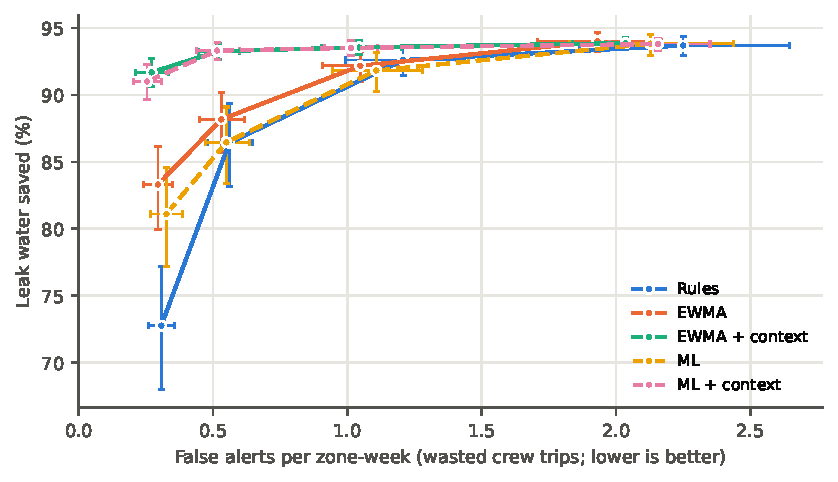
\includegraphics[width=\linewidth]{fig-tradeoff.pdf}
\caption{Share of leaks detected against false alerts per zone-week for alerts after $K = 1, 2, 3$ consecutive alarm hours (larger points: smaller $K$). Horizontal bars: 95\% bootstrap intervals.}
\label{fig:tradeoff}
\end{figure}

\subsection{What causes the false alerts}

Figure~\ref{fig:causes} attributes every false alert to the event active when it started. The model's 652 false alerts are spread over scheduled valve work (118), demand peaks (167), scheduled hydrant tests (71), hours with no event --- mostly hot days with elevated demand (178) --- sensor drift (75) and unscheduled hydrant use (43). The context check removes all false alerts from scheduled work and nearly all from demand (two remain). What it cannot remove is what an operator cannot know in advance: unscheduled hydrant use (44) and part of the sensor drift (44), plus a residue of noise. The rules raise fewer false alerts than the model mainly because they ignore everything with modest flow changes, which is also why they miss small leaks.

\begin{figure}[htbp]
\centering
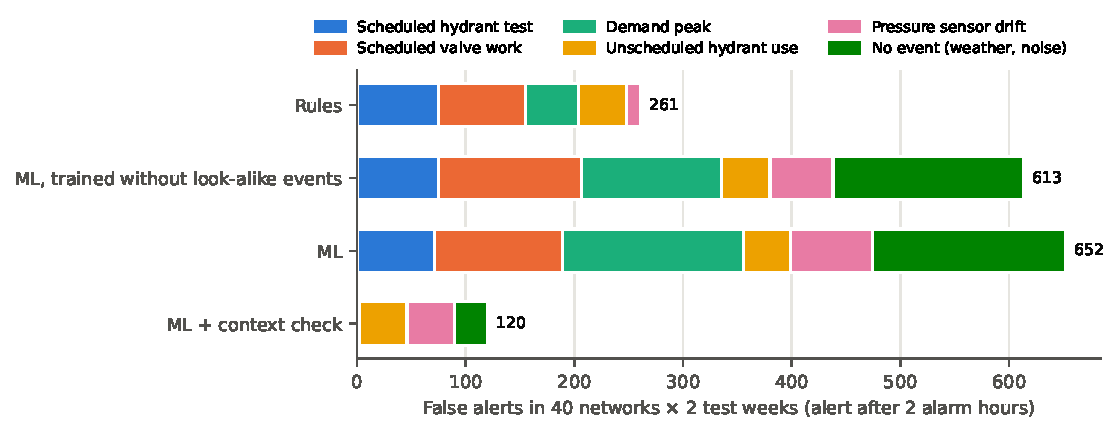
\includegraphics[width=\linewidth]{fig-causes.pdf}
\caption{False alerts in all confirmation networks by the event active when the alert started ($K = 2$).}
\label{fig:causes}
\end{figure}

\subsection{Training with look-alike events (RQ2)}

Training the model with the look-alike events as negative examples did not reduce its false alerts: the difference from the model trained on a leaks-only network is $+0.06$ per zone-week (95\% interval $-0.07$ to $+0.20$). It did reduce sensitivity: 376 instead of 395 leaks detected (paired difference in leak recall $-0.047$, 95\% interval $-0.073$ to $-0.022$). In the feature space of zone telemetry, a valve operation or a demand peak looks like a small leak; labelling them as negatives teaches the model to be less confident about small leaks rather than to recognise the events. The ranking quality of the raw scores agrees: average precision 0.85 for the model and 0.88 for the leaks-only model. The information that separates these events from leaks is not in the readings but in the schedule and the weather, which is what the context check uses.

\subsection{An example week}

Figure~\ref{fig:example} shows one zone during a test week of the demonstration network. A leak at the start of the week is detected by all three methods within two hours. A short unscheduled hydrant draw at hour 82 produces a brief alert from the model, with and without the context check, because nothing an operator knows explains it. A drifting pressure sensor at the end of the week produces a long false alert from the model; the context check recognises a pressure deficit without extra flow and sets it aside, and the rules ignore it because flow is normal.

\begin{figure}[htbp]
\centering
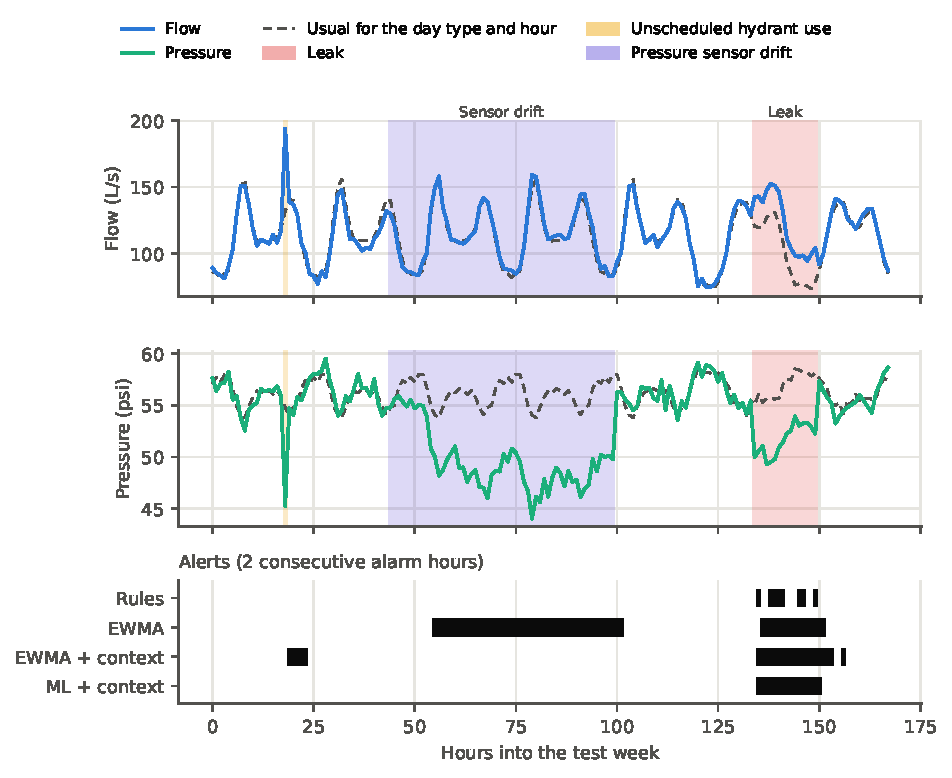
\includegraphics[width=\linewidth]{fig-example.pdf}
\caption{One zone in the test week of the demonstration network: flow and pressure with the usual values for each hour (dashed), true events (shaded), and the alerts of each method.}
\label{fig:example}
\end{figure}

%======================================================================
\section{The dashboard}
\label{sec:app}

The \appname{} is a static web application (Leaflet, Chart.js, ES modules) that runs in the browser without a server and shares its simulator, detectors and measures with the evaluation scripts. \emph{Generate Data} simulates 28 days for the demonstration network; \emph{Train Model} fits the baseline and model on days 1--21 and reports, for the selected method, the leaks detected and false alerts on days 22--28 (Figure~\ref{fig:overview}). The live simulation advances one network hour per tick for all zones and continues the same seeded history.

\begin{figure}[htbp]
\centering
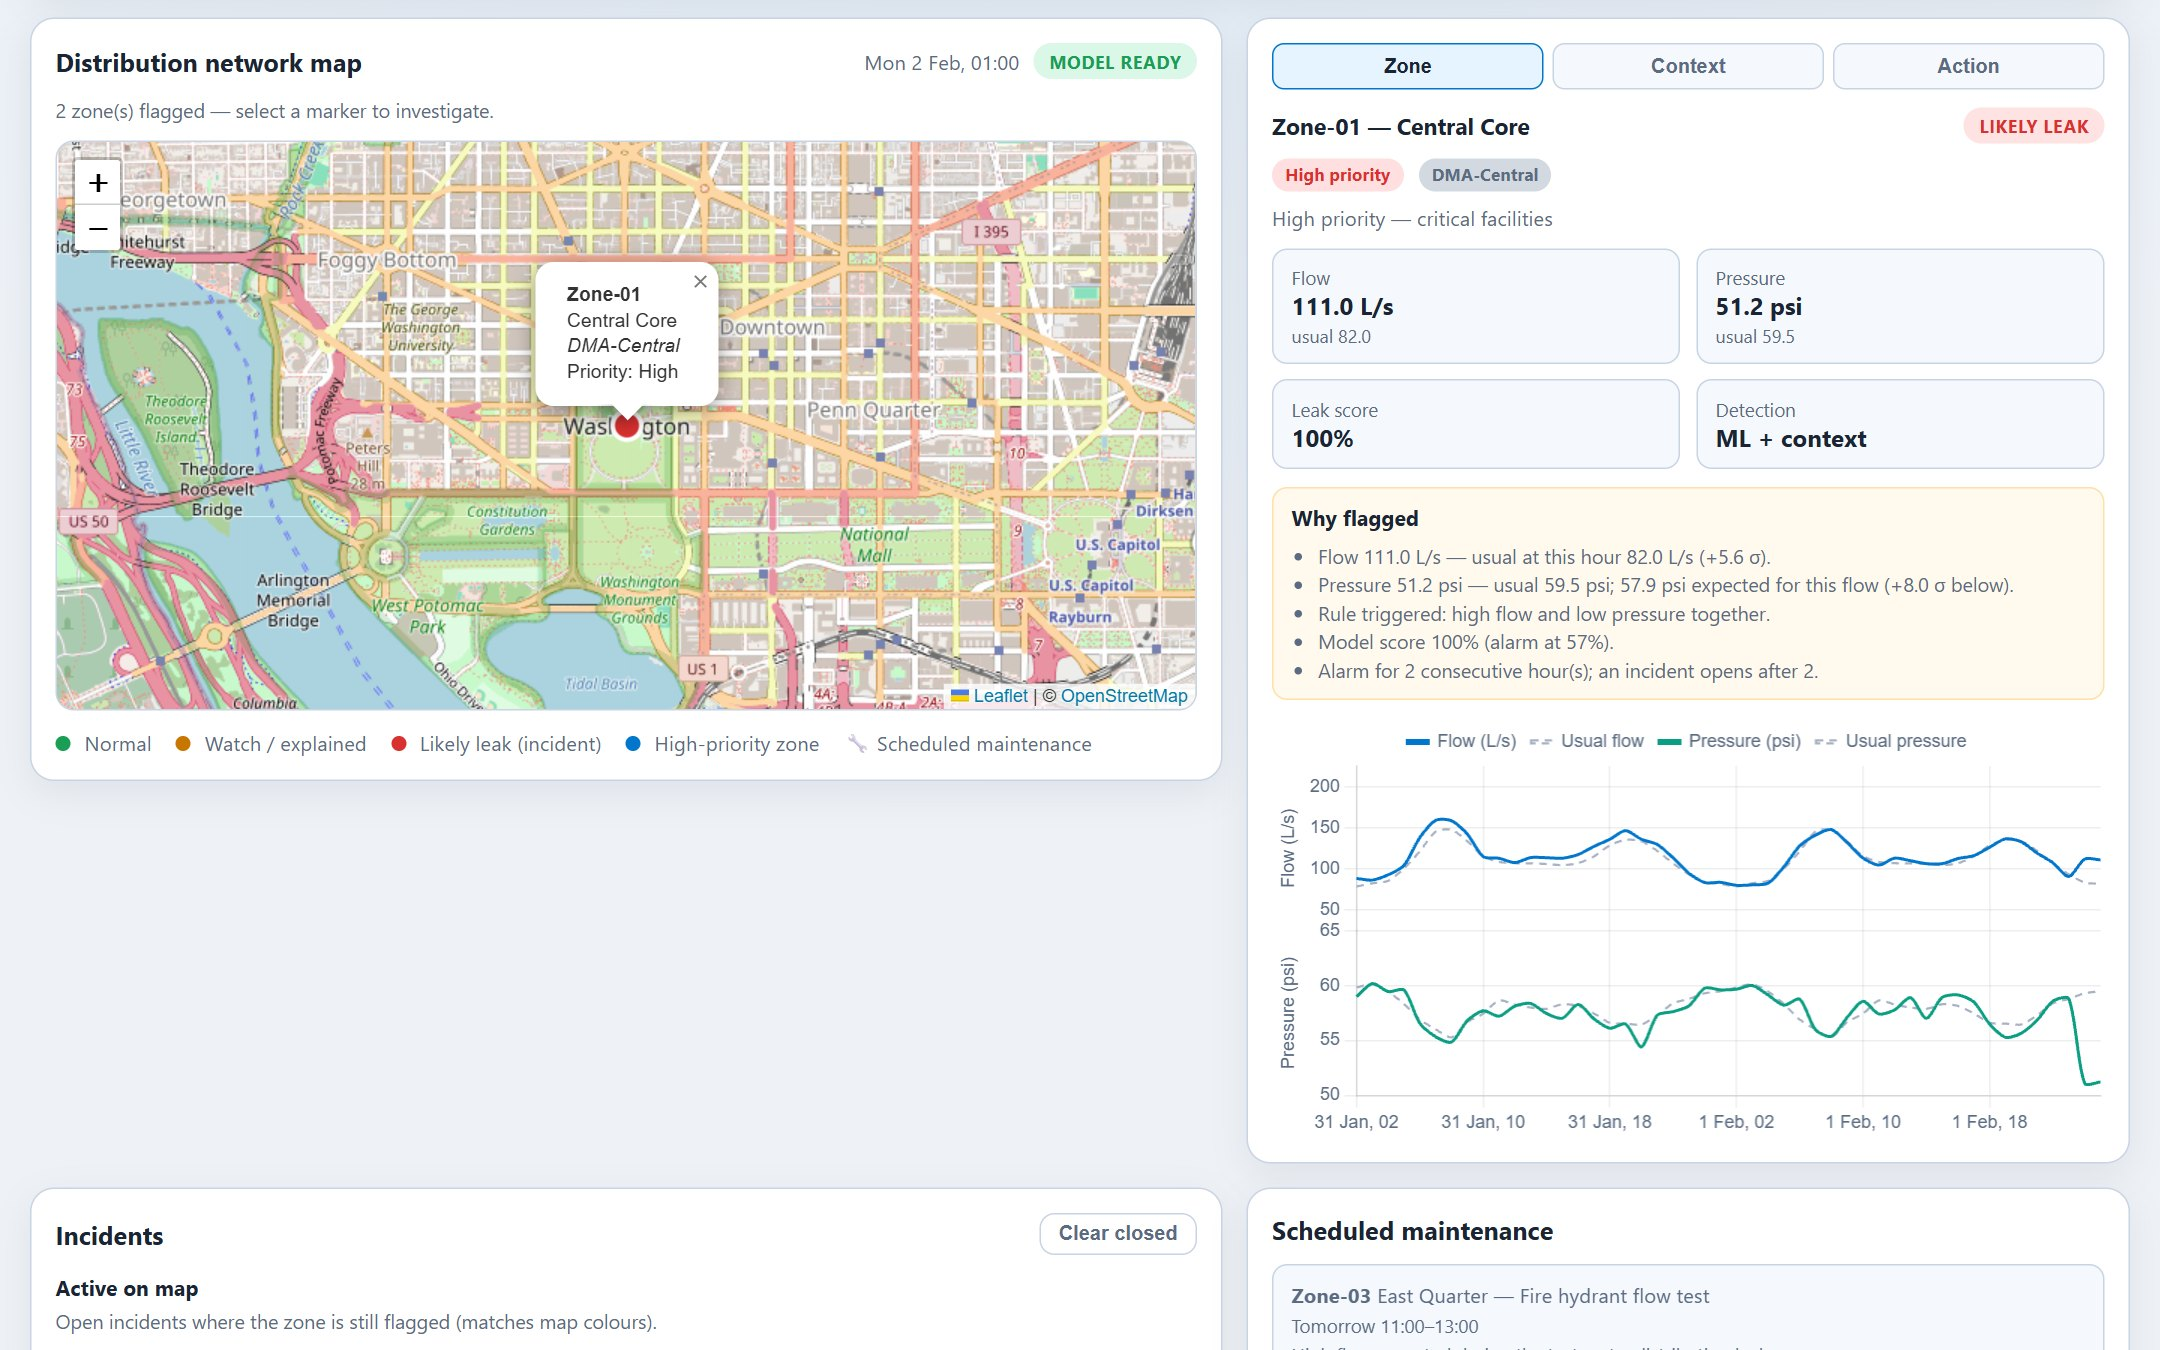
\includegraphics[width=\linewidth]{app-zone.jpg}
\caption{Zone inspector during a leak: flow and pressure against the usual values for the hour, the reasons for the alarm and two stacked history panels with the usual values dashed.}
\label{fig:overview}
\end{figure}

Three design decisions follow from the study. First, an incident opens only after two consecutive abnormal hours, and an incident nobody has acted on closes itself after three normal hours, so short excursions do not accumulate as open cases. Second, the Context tab shows only what an operator has: the network time and its demand period, the day's weather, the zone's published schedule and the result of the context check (Figure~\ref{fig:context}). Third, after an operator closes a case --- as a confirmed leak or as a false alarm --- the dashboard reveals what the simulation contained, states whether the decision was right, and keeps a running score (Figure~\ref{fig:workflow}). Confirming a leak repairs it in the simulation; dismissing a real leak leaves it running, so it alarms again.

\begin{figure}[htbp]
\centering
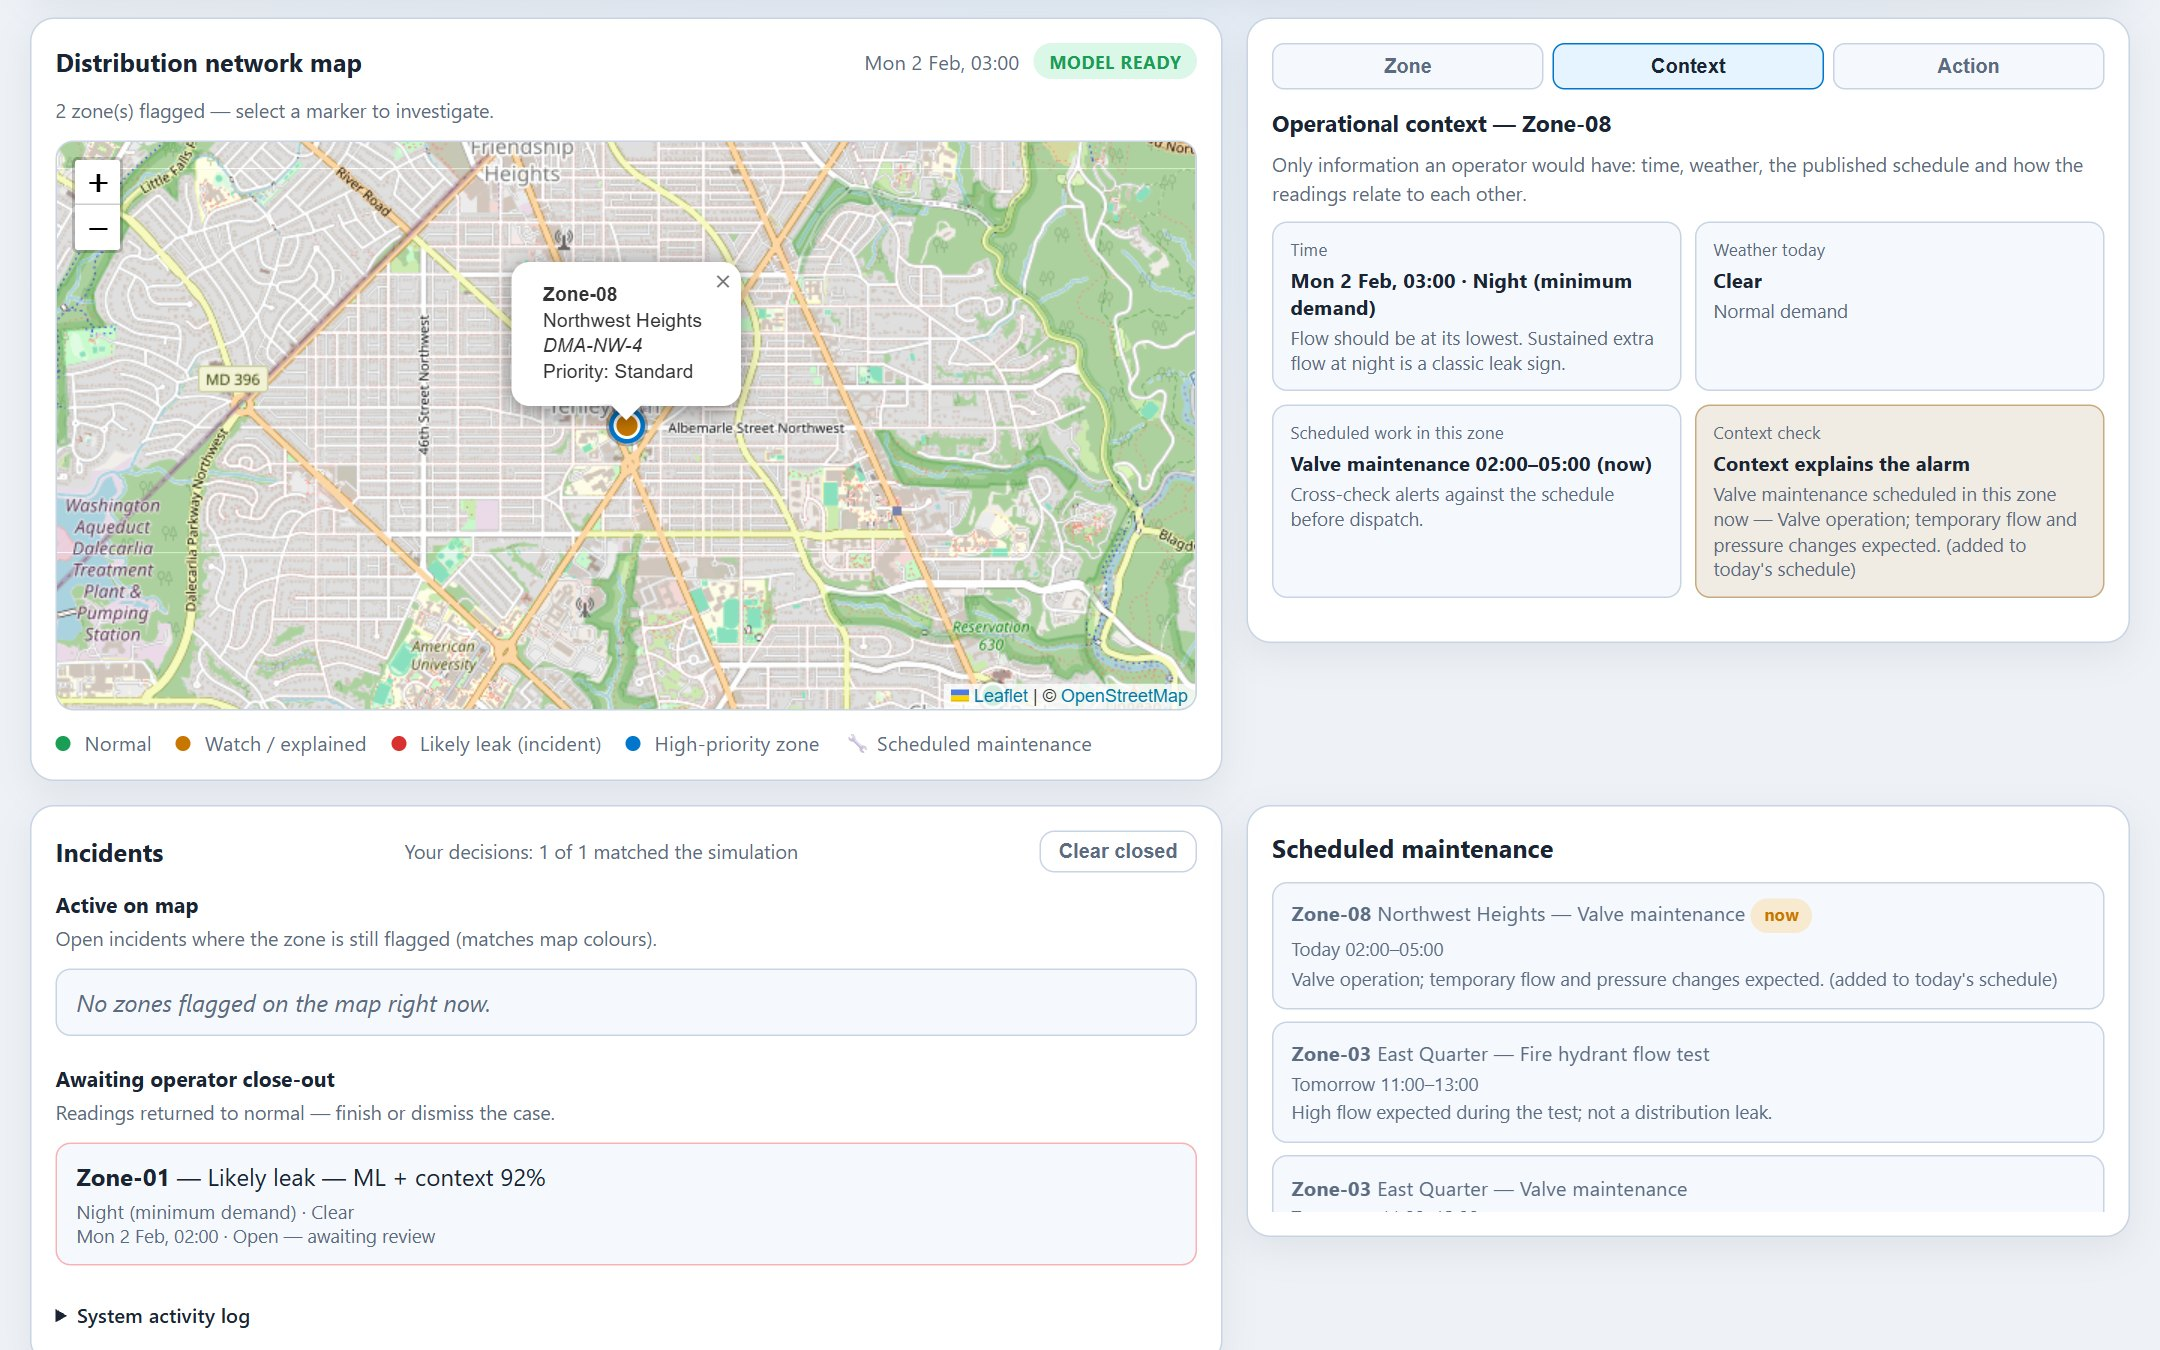
\includegraphics[width=\linewidth]{app-context.jpg}
\caption{Context tab for scheduled valve work: the alarm is explained by the published schedule, so no incident opens.}
\label{fig:context}
\end{figure}

\begin{figure}[htbp]
\centering
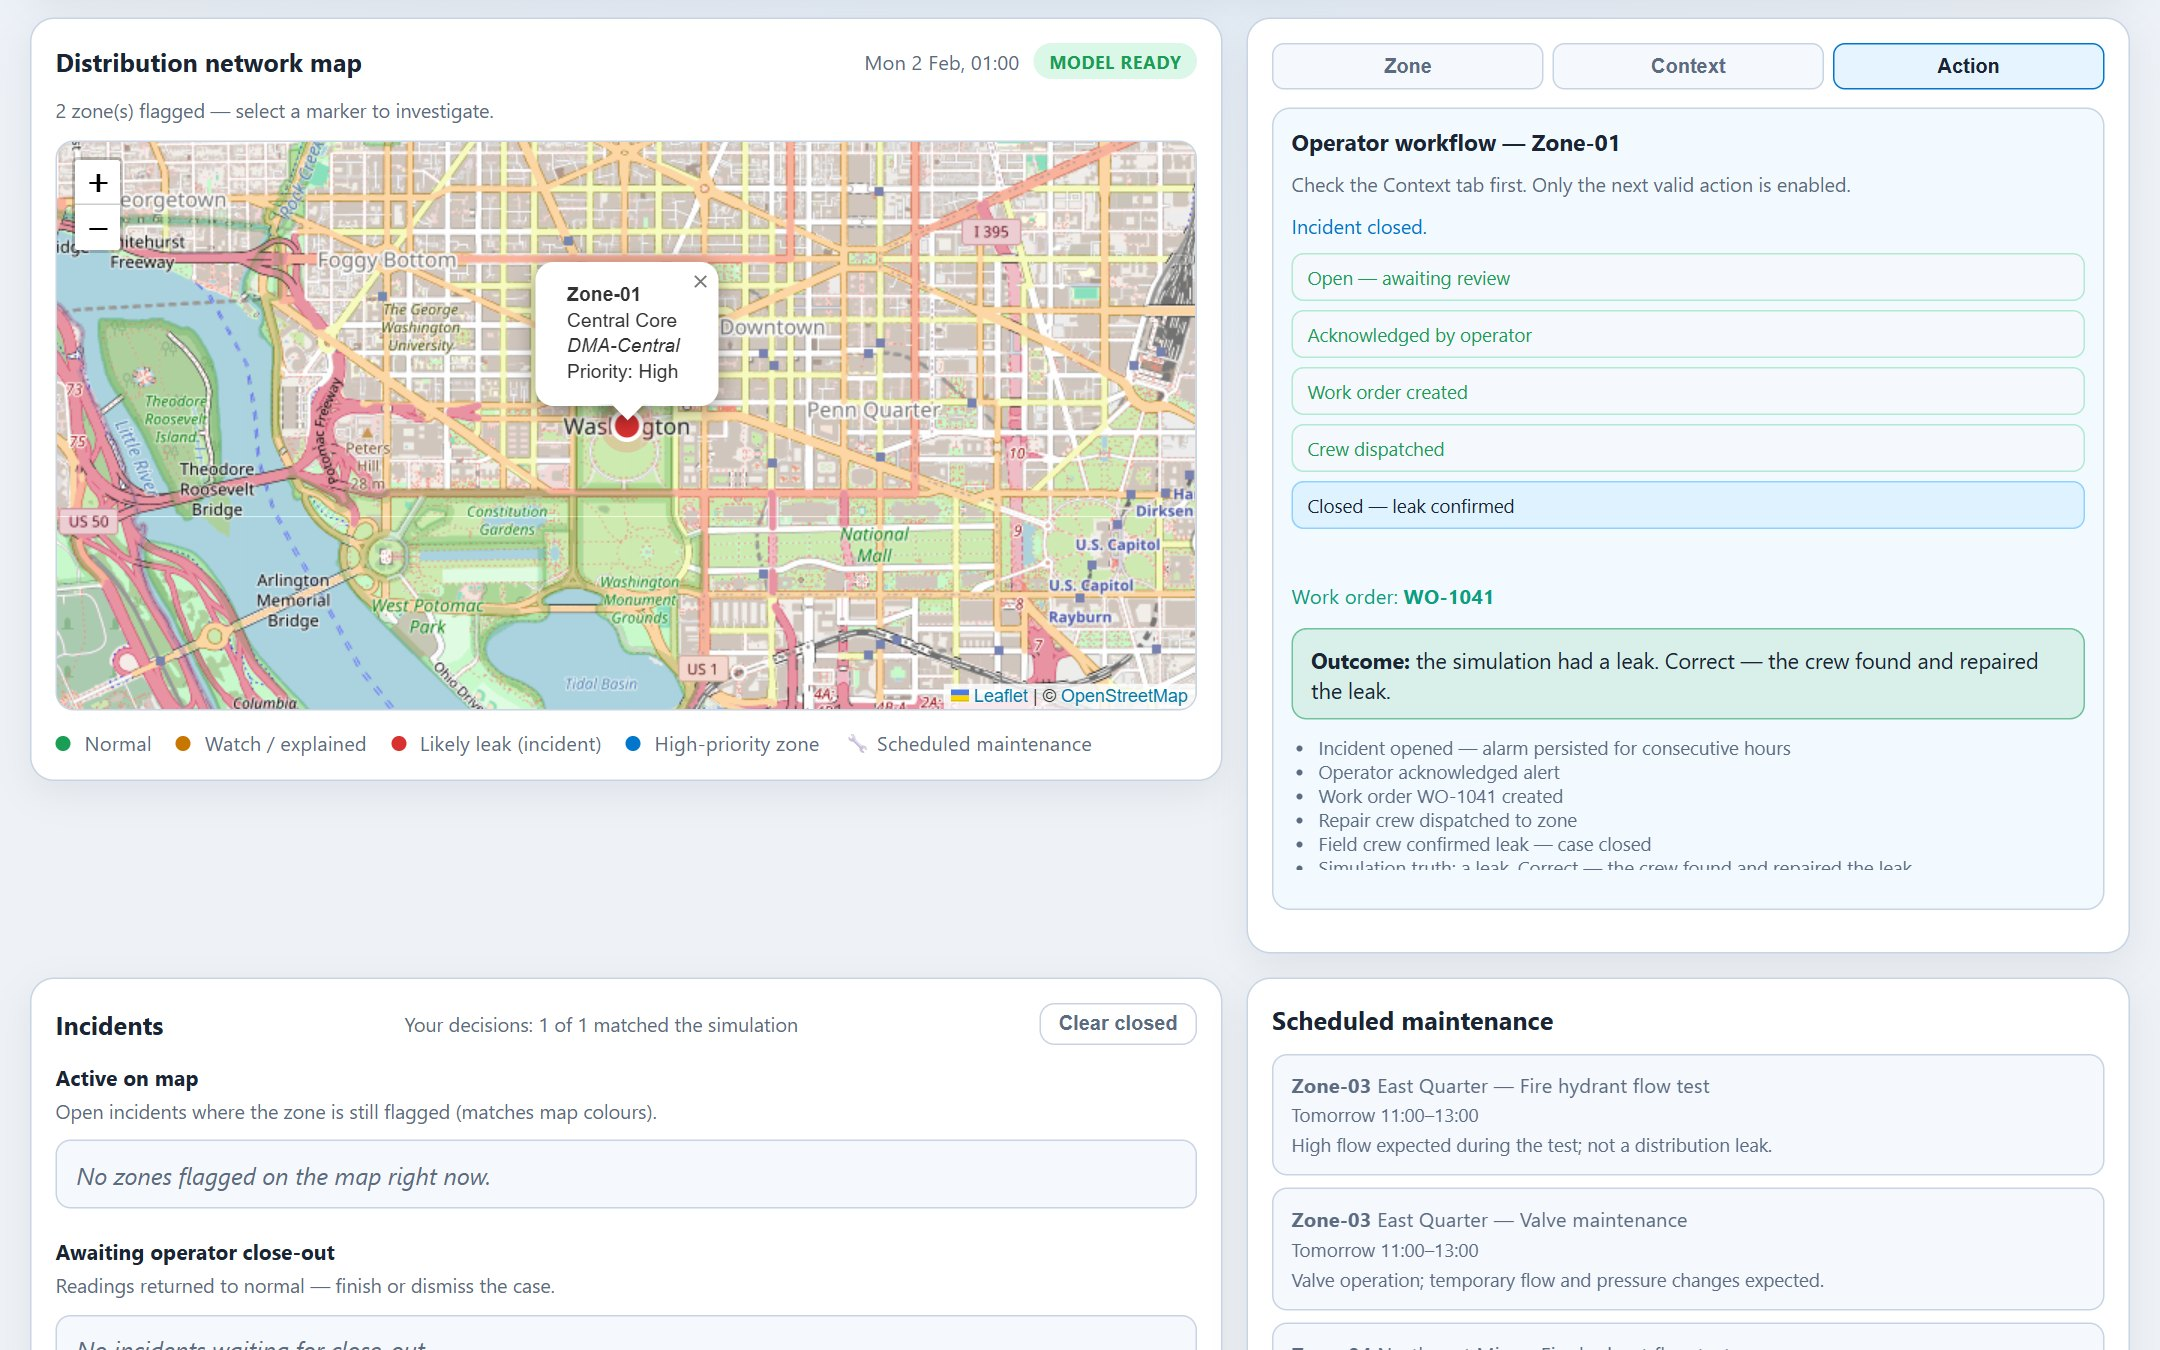
\includegraphics[width=\linewidth]{app-workflow.jpg}
\caption{A closed incident: workflow steps, work order, and the outcome revealed after the decision.}
\label{fig:workflow}
\end{figure}

The dashboard has light and dark themes (the map stays light), a ten-step interactive guide, and phone layouts in which the map follows the controls and touch targets are at least 44\,px (Figure~\ref{fig:phone}). Seventeen unit tests cover the simulator (determinism, schedule consistency, leak persistence and repair, demand profile), the detectors (rules, model, context check, deterministic training, no access to the truth), the measures and the workflow.

\begin{figure}[htbp]
\centering
\begin{subfigure}{0.31\linewidth}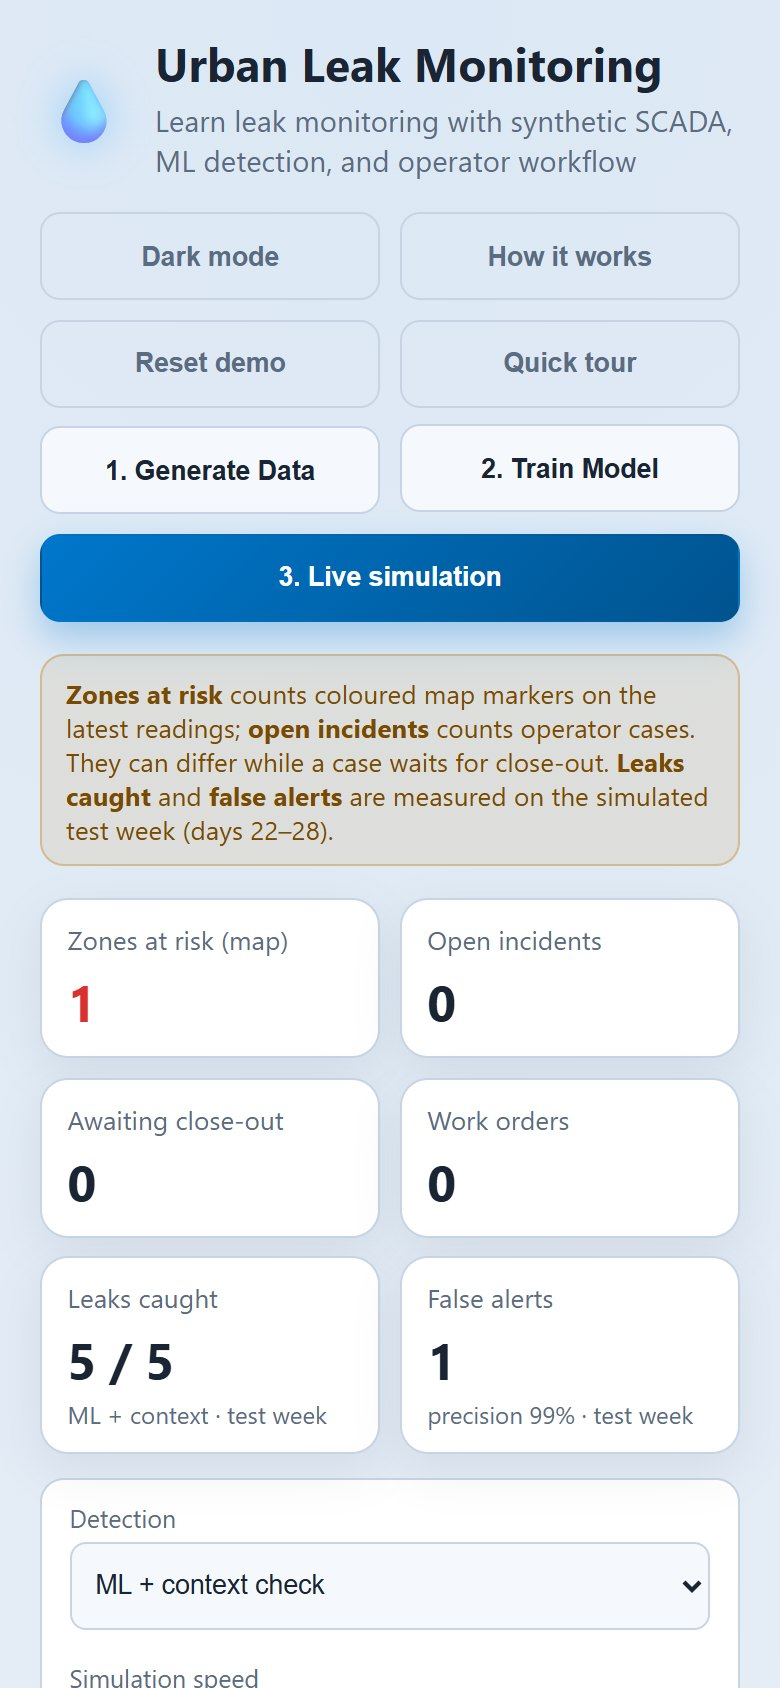
\includegraphics[width=\linewidth]{phone-top.jpg}\caption{Controls and test-week results}\end{subfigure}\hfill
\begin{subfigure}{0.31\linewidth}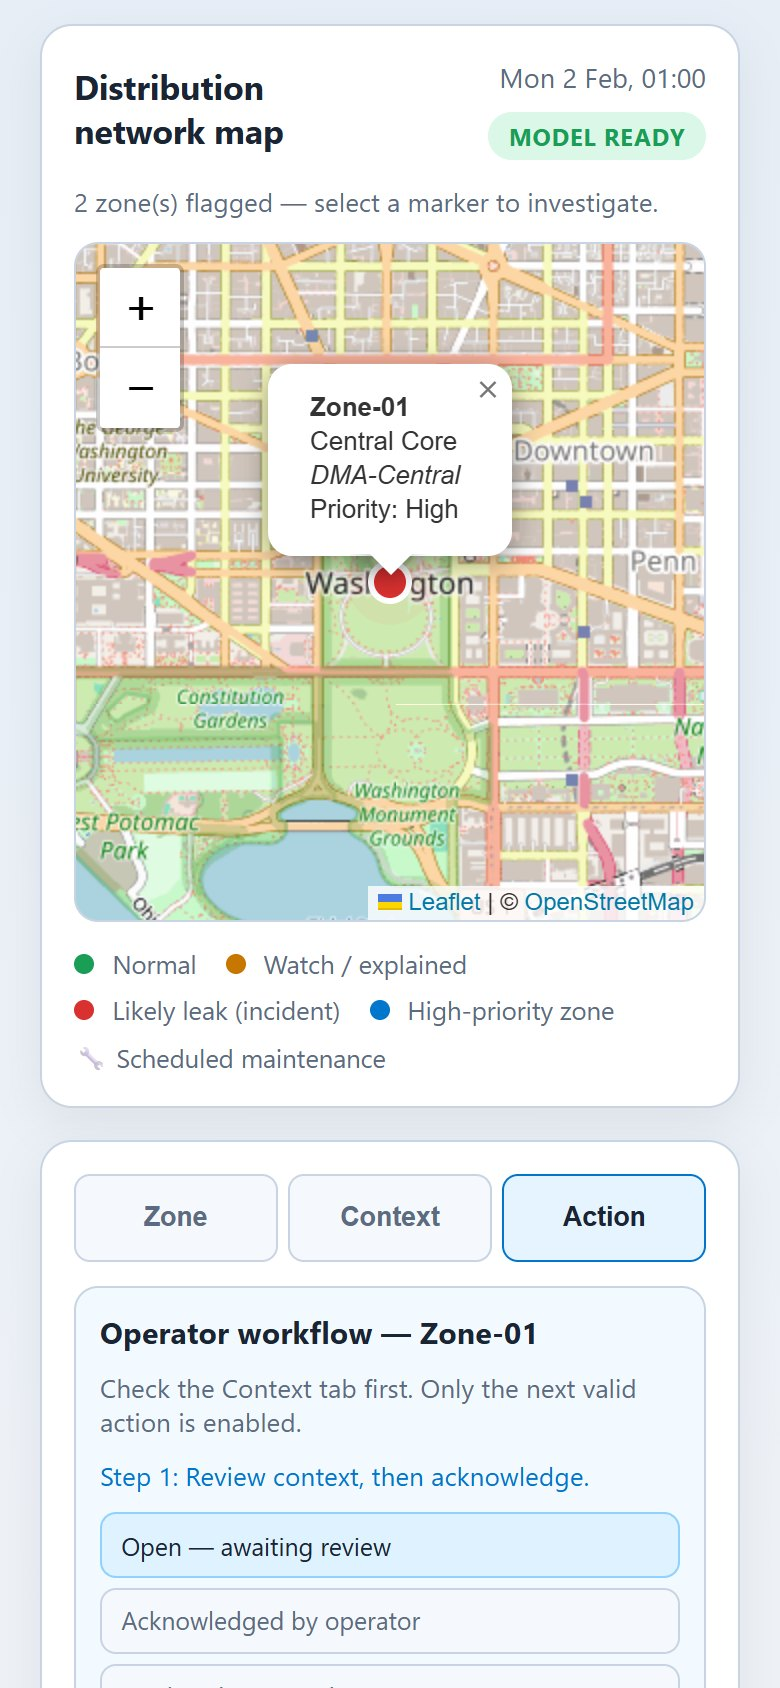
\includegraphics[width=\linewidth]{phone-map.jpg}\caption{Map with a flagged zone}\end{subfigure}\hfill
\begin{subfigure}{0.31\linewidth}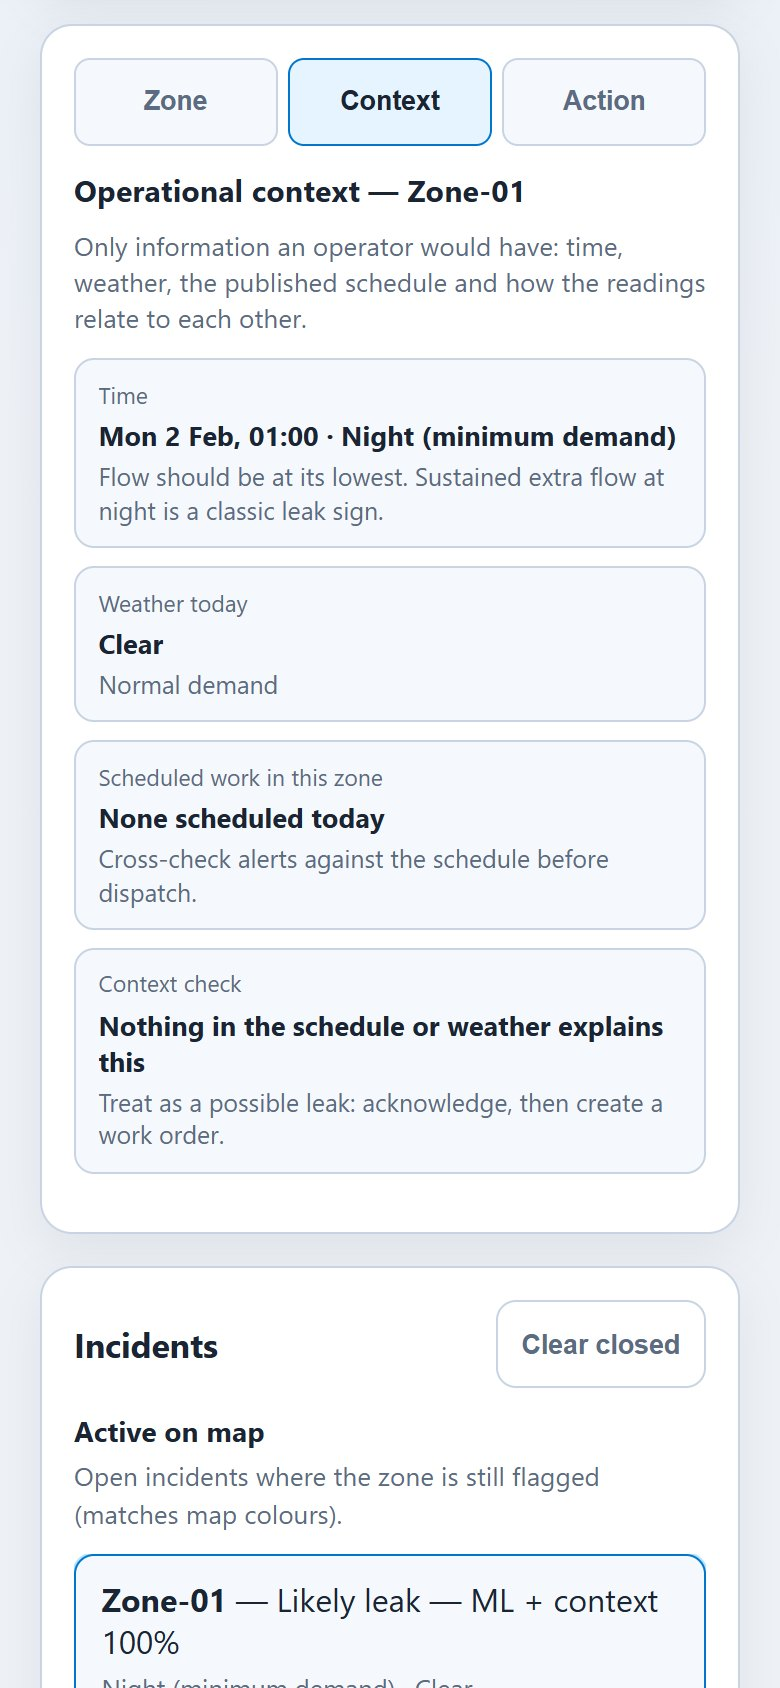
\includegraphics[width=\linewidth]{phone-context.jpg}\caption{Context tab}\end{subfigure}
\caption{Phone layout (390\,px wide).}
\label{fig:phone}
\end{figure}

%======================================================================
\section{Discussion}

\paragraph{Where the information is.} The central result is that the false alerts of a reasonable leak detector are dominated by events that the detector cannot tell apart from leaks but an operator could, from the maintenance schedule and the weather. Adding these events to the training data did not help the model, while consulting the same information an operator has removed four in five false alerts. For practice, this argues for connecting alarm systems to work-order and schedule systems before investing in more complex detectors, and for presenting that context next to every alarm.

\paragraph{Rules versus learning.} The rules were the most precise single detector but missed small leaks, which are the most common and, over time, the most costly. The learned model recovered most of them. Neither alone gave an acceptable balance; the combination did.

\paragraph{Persistence.} Waiting for a second abnormal hour reduced the false alerts of every method by between a third (learned model) and three quarters (with the context check), for a one-hour delay. For leaks that persist for days, this delay is small; for large bursts with immediate safety consequences, a separate high-threshold, no-delay rule would be appropriate.

\paragraph{Limitations.} The network and its parameters are synthetic and were chosen by the author; real networks have weekly cycles, seasonal trends, customer meters and interactions between zones that are not modelled. Detection is per zone, without hydraulic modelling or localisation. The context check is hand-made; its demand rule was refined on the development networks before the confirmation run, and real schedules are incomplete and sometimes wrong, which would reduce its benefit. The results should therefore be read as a controlled comparison of methods and of where information lies, not as performance estimates for a real utility.

\paragraph{Ethics and scope.} The dashboard is a teaching tool. Its map is an OpenStreetMap basemap used for illustration; zone names, network and readings are fictional, and nothing in it describes or evaluates any real utility.

%======================================================================
\section{Conclusion}

In 40 simulated networks with 400 leaks, a learned detector found more leaks than threshold rules but raised two and a half times as many false alerts, and most of those false alerts came from planned work and hot-weather demand. Training with these events did not help; checking the published schedule, the weather and whether pressure fits the flow removed 81\% of the false alerts at a cost of 7 of 400 leaks. The dashboard turns this into practice for learners: alerts that persist, context that an operator really has, and an honest reveal of the truth only after the decision.

\section*{Data and code availability}

\begin{itemize}[leftmargin=1.2em]
  \item Source code, tests, simulation study, figures and this paper: \url{\repourl}\archivedoi
  \item Live dashboard: \url{\appurl}
  \item Reproduce the study (about seven seconds; all data are simulated):\\ \texttt{node evaluation/run\_experiments.mjs}
\end{itemize}

%======================================================================
\begin{thebibliography}{99}
\small

\bibitem{bainbridge1983} L.~Bainbridge, ``Ironies of automation,'' \emph{Automatica}, vol.~19, no.~6, pp.~775--779, 1983.

\bibitem{colombo2009} A.~F. Colombo, P.~Lee, and B.~W. Karney, ``A selective literature review of transient-based leak detection methods,'' \emph{Journal of Hydro-environment Research}, vol.~2, no.~4, pp.~212--227, 2009.

\bibitem{cvach2012} M.~Cvach, ``Monitor alarm fatigue: An integrative review,'' \emph{Biomedical Instrumentation \& Technology}, vol.~46, no.~4, pp.~268--277, 2012.

\bibitem{farley2003} M.~Farley and S.~Trow, \emph{Losses in Water Distribution Networks: A Practitioner's Guide to Assessment, Monitoring and Control}. London: IWA Publishing, 2003.

\bibitem{kleiner2001} Y.~Kleiner and B.~Rajani, ``Comprehensive review of structural deterioration of water mains: Statistical models,'' \emph{Urban Water}, vol.~3, no.~3, pp.~131--150, 2001.

\bibitem{lambert2002} A.~O. Lambert, ``International report: Water losses management and techniques,'' \emph{Water Science and Technology: Water Supply}, vol.~2, no.~4, pp.~1--20, 2002.

\bibitem{leys2013} C.~Leys, C.~Ley, O.~Klein, P.~Bernard, and L.~Licata, ``Detecting outliers: Do not use standard deviation around the mean, use absolute deviation around the median,'' \emph{Journal of Experimental Social Psychology}, vol.~49, no.~4, pp.~764--766, 2013.

\bibitem{mounce2010} S.~R. Mounce, J.~B. Boxall, and J.~Machell, ``Development and verification of an online artificial intelligence system for detection of bursts and other abnormal flows,'' \emph{Journal of Water Resources Planning and Management}, vol.~136, no.~3, pp.~309--318, 2010.

\bibitem{parasuraman1997} R.~Parasuraman and V.~Riley, ``Humans and automation: Use, misuse, disuse, abuse,'' \emph{Human Factors}, vol.~39, no.~2, pp.~230--253, 1997.

\bibitem{puust2010} R.~Puust, Z.~Kapelan, D.~A. Savi\'{c}, and T.~Koppel, ``A review of methods for leakage management in pipe networks,'' \emph{Urban Water Journal}, vol.~7, no.~1, pp.~25--45, 2010.

\bibitem{romano2014} M.~Romano, Z.~Kapelan, and D.~A. Savi\'{c}, ``Automated detection of pipe bursts and other events in water distribution systems,'' \emph{Journal of Water Resources Planning and Management}, vol.~140, no.~4, pp.~457--467, 2014.

\bibitem{saito2015} T.~Saito and M.~Rehmsmeier, ``The precision-recall plot is more informative than the ROC plot when evaluating binary classifiers on imbalanced datasets,'' \emph{PLoS ONE}, vol.~10, no.~3, e0118432, 2015.

\bibitem{wickens2007} C.~D. Wickens and S.~R. Dixon, ``The benefits of imperfect diagnostic automation: A synthesis of the literature,'' \emph{Theoretical Issues in Ergonomics Science}, vol.~8, no.~3, pp.~201--212, 2007.

\bibitem{wu2017} Y.~Wu and S.~Liu, ``A review of data-driven approaches for burst detection in water distribution systems,'' \emph{Urban Water Journal}, vol.~14, no.~9, pp.~972--983, 2017.

\end{thebibliography}

\end{document}
